\documentclass[twoside]{book}

% Packages required by doxygen
\usepackage{fixltx2e}
\usepackage{calc}
\usepackage{doxygen}
\usepackage[export]{adjustbox} % also loads graphicx
\usepackage{graphicx}
\usepackage[utf8]{inputenc}
\usepackage{makeidx}
\usepackage{multicol}
\usepackage{multirow}
\PassOptionsToPackage{warn}{textcomp}
\usepackage{textcomp}
\usepackage[nointegrals]{wasysym}
\usepackage[table]{xcolor}

% Font selection
\usepackage[T1]{fontenc}
\usepackage[scaled=.90]{helvet}
\usepackage{courier}
\usepackage{amssymb}
\usepackage{sectsty}
\renewcommand{\familydefault}{\sfdefault}
\allsectionsfont{%
  \fontseries{bc}\selectfont%
  \color{darkgray}%
}
\renewcommand{\DoxyLabelFont}{%
  \fontseries{bc}\selectfont%
  \color{darkgray}%
}
\newcommand{\+}{\discretionary{\mbox{\scriptsize$\hookleftarrow$}}{}{}}

% Page & text layout
\usepackage{geometry}
\geometry{%
  a4paper,%
  top=2.5cm,%
  bottom=2.5cm,%
  left=2.5cm,%
  right=2.5cm%
}
\tolerance=750
\hfuzz=15pt
\hbadness=750
\setlength{\emergencystretch}{15pt}
\setlength{\parindent}{0cm}
\setlength{\parskip}{3ex plus 2ex minus 2ex}
\makeatletter
\renewcommand{\paragraph}{%
  \@startsection{paragraph}{4}{0ex}{-1.0ex}{1.0ex}{%
    \normalfont\normalsize\bfseries\SS@parafont%
  }%
}
\renewcommand{\subparagraph}{%
  \@startsection{subparagraph}{5}{0ex}{-1.0ex}{1.0ex}{%
    \normalfont\normalsize\bfseries\SS@subparafont%
  }%
}
\makeatother

% Headers & footers
\usepackage{fancyhdr}
\pagestyle{fancyplain}
\fancyhead[LE]{\fancyplain{}{\bfseries\thepage}}
\fancyhead[CE]{\fancyplain{}{}}
\fancyhead[RE]{\fancyplain{}{\bfseries\leftmark}}
\fancyhead[LO]{\fancyplain{}{\bfseries\rightmark}}
\fancyhead[CO]{\fancyplain{}{}}
\fancyhead[RO]{\fancyplain{}{\bfseries\thepage}}
\fancyfoot[LE]{\fancyplain{}{}}
\fancyfoot[CE]{\fancyplain{}{}}
\fancyfoot[RE]{\fancyplain{}{\bfseries\scriptsize Generated by Doxygen }}
\fancyfoot[LO]{\fancyplain{}{\bfseries\scriptsize Generated by Doxygen }}
\fancyfoot[CO]{\fancyplain{}{}}
\fancyfoot[RO]{\fancyplain{}{}}
\renewcommand{\footrulewidth}{0.4pt}
\renewcommand{\chaptermark}[1]{%
  \markboth{#1}{}%
}
\renewcommand{\sectionmark}[1]{%
  \markright{\thesection\ #1}%
}

% Indices & bibliography
\usepackage{natbib}
\usepackage[titles]{tocloft}
\setcounter{tocdepth}{3}
\setcounter{secnumdepth}{5}
\makeindex

% Hyperlinks (required, but should be loaded last)
\usepackage{ifpdf}
\ifpdf
  \usepackage[pdftex,pagebackref=true]{hyperref}
\else
  \usepackage[ps2pdf,pagebackref=true]{hyperref}
\fi
\hypersetup{%
  colorlinks=true,%
  linkcolor=blue,%
  citecolor=blue,%
  unicode%
}

% Custom commands
\newcommand{\clearemptydoublepage}{%
  \newpage{\pagestyle{empty}\cleardoublepage}%
}

\usepackage{caption}
\captionsetup{labelsep=space,justification=centering,font={bf},singlelinecheck=off,skip=4pt,position=top}

%===== C O N T E N T S =====

\begin{document}

% Titlepage & ToC
\hypersetup{pageanchor=false,
             bookmarksnumbered=true,
             pdfencoding=unicode
            }
\pagenumbering{roman}
\begin{titlepage}
\vspace*{7cm}
\begin{center}%
{\Large My Project }\\
\vspace*{1cm}
{\large Generated by Doxygen 1.8.11}\\
\end{center}
\end{titlepage}
\clearemptydoublepage
\tableofcontents
\clearemptydoublepage
\pagenumbering{arabic}
\hypersetup{pageanchor=true}

%--- Begin generated contents ---
\chapter{Class Index}
\section{Class List}
Here are the classes, structs, unions and interfaces with brief descriptions\+:\begin{DoxyCompactList}
\item\contentsline{section}{\hyperlink{structnode}{node} }{\pageref{structnode}}{}
\item\contentsline{section}{\hyperlink{structnode1}{node1} }{\pageref{structnode1}}{}
\item\contentsline{section}{\hyperlink{structnode__info}{node\+\_\+info} }{\pageref{structnode__info}}{}
\end{DoxyCompactList}

\chapter{File Index}
\section{File List}
Here is a list of all files with brief descriptions\+:\begin{DoxyCompactList}
\item\contentsline{section}{\hyperlink{Lab1_8c}{Lab1.\+c} }{\pageref{Lab1_8c}}{}
\end{DoxyCompactList}

\chapter{Class Documentation}
\hypertarget{structnode}{}\section{node Struct Reference}
\label{structnode}\index{node@{node}}


Collaboration diagram for node\+:
\nopagebreak
\begin{figure}[H]
\begin{center}
\leavevmode
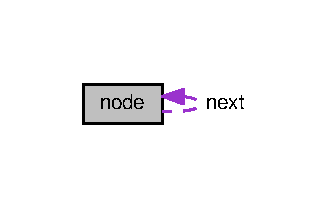
\includegraphics[width=158pt]{structnode__coll__graph}
\end{center}
\end{figure}
\subsection*{Public Attributes}
\begin{DoxyCompactItemize}
\item 
int \hyperlink{structnode_a2d890bb9f6af0ffd73fe79b21124c2a2}{data}
\item 
\hyperlink{structnode}{node} $\ast$ \hyperlink{structnode_aad210fa7c160a49f6b9a3ffee592a2bc}{next}
\end{DoxyCompactItemize}


\subsection{Member Data Documentation}
\index{node@{node}!data@{data}}
\index{data@{data}!node@{node}}
\subsubsection[{\texorpdfstring{data}{data}}]{\setlength{\rightskip}{0pt plus 5cm}int node\+::data}\hypertarget{structnode_a2d890bb9f6af0ffd73fe79b21124c2a2}{}\label{structnode_a2d890bb9f6af0ffd73fe79b21124c2a2}
\index{node@{node}!next@{next}}
\index{next@{next}!node@{node}}
\subsubsection[{\texorpdfstring{next}{next}}]{\setlength{\rightskip}{0pt plus 5cm}{\bf node}$\ast$ node\+::next}\hypertarget{structnode_aad210fa7c160a49f6b9a3ffee592a2bc}{}\label{structnode_aad210fa7c160a49f6b9a3ffee592a2bc}


The documentation for this struct was generated from the following file\+:\begin{DoxyCompactItemize}
\item 
\hyperlink{SelfOrganizing_8cpp}{Self\+Organizing.\+cpp}\end{DoxyCompactItemize}

\chapter{File Documentation}
\hypertarget{SelfOrganizing_8cpp}{}\section{Self\+Organizing.\+cpp File Reference}
\label{SelfOrganizing_8cpp}\index{Self\+Organizing.\+cpp@{Self\+Organizing.\+cpp}}
{\ttfamily \#include $<$iostream$>$}\\*
Include dependency graph for Self\+Organizing.\+cpp\+:
\nopagebreak
\begin{figure}[H]
\begin{center}
\leavevmode
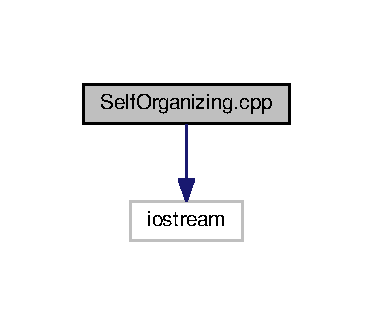
\includegraphics[width=179pt]{SelfOrganizing_8cpp__incl}
\end{center}
\end{figure}
\subsection*{Classes}
\begin{DoxyCompactItemize}
\item 
struct \hyperlink{structnode}{node}
\end{DoxyCompactItemize}
\subsection*{Functions}
\begin{DoxyCompactItemize}
\item 
\hyperlink{structnode}{node} $\ast$ \hyperlink{SelfOrganizing_8cpp_acdfbac0b55098c103f6996cb5c8333a9}{Create\+Node} (int data)
\item 
\hyperlink{structnode}{node} $\ast$ \hyperlink{SelfOrganizing_8cpp_afc94029a35bc1927140eddfb87f5a4d7}{Insert\+Into\+List} (\hyperlink{structnode}{node} $\ast$head, int data)
\item 
void \hyperlink{SelfOrganizing_8cpp_a2c91327d8e8e4b94626520b4877a4cff}{Display} (\hyperlink{structnode}{node} $\ast$head)
\item 
\hyperlink{structnode}{node} $\ast$ \hyperlink{SelfOrganizing_8cpp_ad3123efb060bc3f8c45bd4f15b25bf3e}{Search\+Item} (\hyperlink{structnode}{node} $\ast$head, int item)
\item 
int \hyperlink{SelfOrganizing_8cpp_ae66f6b31b5ad750f1fe042a706a4e3d4}{main} ()
\end{DoxyCompactItemize}


\subsection{Function Documentation}
\index{Self\+Organizing.\+cpp@{Self\+Organizing.\+cpp}!Create\+Node@{Create\+Node}}
\index{Create\+Node@{Create\+Node}!Self\+Organizing.\+cpp@{Self\+Organizing.\+cpp}}
\subsubsection[{\texorpdfstring{Create\+Node(int data)}{CreateNode(int data)}}]{\setlength{\rightskip}{0pt plus 5cm}{\bf node}$\ast$ Create\+Node (
\begin{DoxyParamCaption}
\item[{int}]{data}
\end{DoxyParamCaption}
)}\hypertarget{SelfOrganizing_8cpp_acdfbac0b55098c103f6996cb5c8333a9}{}\label{SelfOrganizing_8cpp_acdfbac0b55098c103f6996cb5c8333a9}

\begin{DoxyCode}
14 \{
15     \hyperlink{structnode}{node} *newnode = \textcolor{keyword}{new} \hyperlink{structnode}{node};
16     newnode->\hyperlink{structnode_a2d890bb9f6af0ffd73fe79b21124c2a2}{data} = data;
17     newnode->\hyperlink{structnode_aad210fa7c160a49f6b9a3ffee592a2bc}{next} = NULL;
18     \textcolor{keywordflow}{return} newnode;
19 \}
\end{DoxyCode}
\index{Self\+Organizing.\+cpp@{Self\+Organizing.\+cpp}!Display@{Display}}
\index{Display@{Display}!Self\+Organizing.\+cpp@{Self\+Organizing.\+cpp}}
\subsubsection[{\texorpdfstring{Display(node $\ast$head)}{Display(node *head)}}]{\setlength{\rightskip}{0pt plus 5cm}void Display (
\begin{DoxyParamCaption}
\item[{{\bf node} $\ast$}]{head}
\end{DoxyParamCaption}
)}\hypertarget{SelfOrganizing_8cpp_a2c91327d8e8e4b94626520b4877a4cff}{}\label{SelfOrganizing_8cpp_a2c91327d8e8e4b94626520b4877a4cff}

\begin{DoxyCode}
44 \{
45     \hyperlink{structnode}{node} *temp = \textcolor{keyword}{new} \hyperlink{structnode}{node};
46     temp = head;
47     cout<<\textcolor{stringliteral}{"\(\backslash\)n The list state is :"};
48     \textcolor{comment}{// Display the list.}
49     \textcolor{keywordflow}{while}(temp->\hyperlink{structnode_aad210fa7c160a49f6b9a3ffee592a2bc}{next} != NULL)
50     \{
51         cout<<\textcolor{stringliteral}{"->"}<<temp->\hyperlink{structnode_a2d890bb9f6af0ffd73fe79b21124c2a2}{data};
52         temp = temp->\hyperlink{structnode_aad210fa7c160a49f6b9a3ffee592a2bc}{next};
53     \}
54 \}
\end{DoxyCode}
\index{Self\+Organizing.\+cpp@{Self\+Organizing.\+cpp}!Insert\+Into\+List@{Insert\+Into\+List}}
\index{Insert\+Into\+List@{Insert\+Into\+List}!Self\+Organizing.\+cpp@{Self\+Organizing.\+cpp}}
\subsubsection[{\texorpdfstring{Insert\+Into\+List(node $\ast$head, int data)}{InsertIntoList(node *head, int data)}}]{\setlength{\rightskip}{0pt plus 5cm}{\bf node}$\ast$ Insert\+Into\+List (
\begin{DoxyParamCaption}
\item[{{\bf node} $\ast$}]{head, }
\item[{int}]{data}
\end{DoxyParamCaption}
)}\hypertarget{SelfOrganizing_8cpp_afc94029a35bc1927140eddfb87f5a4d7}{}\label{SelfOrganizing_8cpp_afc94029a35bc1927140eddfb87f5a4d7}

\begin{DoxyCode}
23 \{
24     \hyperlink{structnode}{node} *temp = \hyperlink{SelfOrganizing_8cpp_acdfbac0b55098c103f6996cb5c8333a9}{CreateNode}(data);
25     \hyperlink{structnode}{node} *t = \textcolor{keyword}{new} \hyperlink{structnode}{node};
26     t = head;
27     \textcolor{keywordflow}{if}(head == NULL)
28     \{
29         head = temp;
30         \textcolor{keywordflow}{return} head;
31     \}
32     \textcolor{keywordflow}{else}
33     \{
34         \textcolor{comment}{// Traversing to the end of the list.}
35         \textcolor{keywordflow}{while}(t->\hyperlink{structnode_aad210fa7c160a49f6b9a3ffee592a2bc}{next} != NULL)
36             t = t->\hyperlink{structnode_aad210fa7c160a49f6b9a3ffee592a2bc}{next};
37         \textcolor{comment}{// Add the node at the end. }
38         t->\hyperlink{structnode_aad210fa7c160a49f6b9a3ffee592a2bc}{next} = temp;
39     \}
40     \textcolor{keywordflow}{return} head;
41 \}
\end{DoxyCode}


Here is the call graph for this function\+:
\nopagebreak
\begin{figure}[H]
\begin{center}
\leavevmode
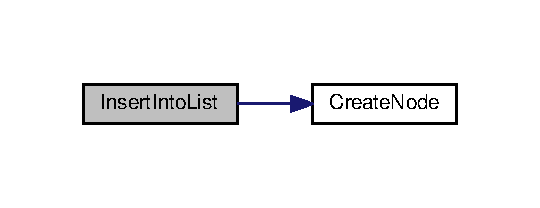
\includegraphics[width=259pt]{SelfOrganizing_8cpp_afc94029a35bc1927140eddfb87f5a4d7_cgraph}
\end{center}
\end{figure}


\index{Self\+Organizing.\+cpp@{Self\+Organizing.\+cpp}!main@{main}}
\index{main@{main}!Self\+Organizing.\+cpp@{Self\+Organizing.\+cpp}}
\subsubsection[{\texorpdfstring{main()}{main()}}]{\setlength{\rightskip}{0pt plus 5cm}int main (
\begin{DoxyParamCaption}
{}
\end{DoxyParamCaption}
)}\hypertarget{SelfOrganizing_8cpp_ae66f6b31b5ad750f1fe042a706a4e3d4}{}\label{SelfOrganizing_8cpp_ae66f6b31b5ad750f1fe042a706a4e3d4}

\begin{DoxyCode}
96 \{
97     \textcolor{keywordtype}{int} i, n;
98     \textcolor{keywordtype}{char} ch;
99     \hyperlink{structnode}{node} *head = \textcolor{keyword}{new} \hyperlink{structnode}{node};
100     head = NULL;
101  
102     \textcolor{keywordflow}{for}(i = 1; i < 11; i++)
103         head = \hyperlink{SelfOrganizing_8cpp_afc94029a35bc1927140eddfb87f5a4d7}{InsertIntoList}(head, i);
104  
105     \hyperlink{SelfOrganizing_8cpp_a2c91327d8e8e4b94626520b4877a4cff}{Display}(head);
106  
107     up:
108     cout<<\textcolor{stringliteral}{"\(\backslash\)nEnter the Element to be searched: "};
109     cin>>n;
110     \textcolor{comment}{// Update the head of the list.}
111     head = \hyperlink{SelfOrganizing_8cpp_ad3123efb060bc3f8c45bd4f15b25bf3e}{SearchItem}(head, n);
112  
113     cout<<\textcolor{stringliteral}{"\(\backslash\)n\(\backslash\)n\(\backslash\)tDo you want to search more...enter choice(y/n)?"};
114     cin>>ch;
115     \textcolor{keywordflow}{if}(ch == \textcolor{charliteral}{'y'} || ch == \textcolor{charliteral}{'Y'})
116     \textcolor{keywordflow}{goto} up;
117  
118     \textcolor{keywordflow}{return} 0;
119 \}\end{DoxyCode}


Here is the call graph for this function\+:
\nopagebreak
\begin{figure}[H]
\begin{center}
\leavevmode
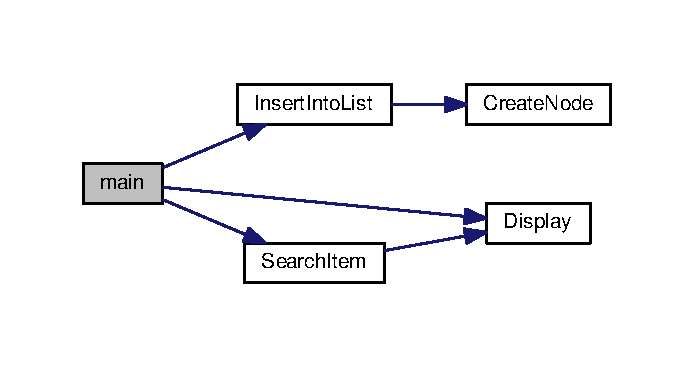
\includegraphics[width=333pt]{SelfOrganizing_8cpp_ae66f6b31b5ad750f1fe042a706a4e3d4_cgraph}
\end{center}
\end{figure}


\index{Self\+Organizing.\+cpp@{Self\+Organizing.\+cpp}!Search\+Item@{Search\+Item}}
\index{Search\+Item@{Search\+Item}!Self\+Organizing.\+cpp@{Self\+Organizing.\+cpp}}
\subsubsection[{\texorpdfstring{Search\+Item(node $\ast$head, int item)}{SearchItem(node *head, int item)}}]{\setlength{\rightskip}{0pt plus 5cm}{\bf node}$\ast$ Search\+Item (
\begin{DoxyParamCaption}
\item[{{\bf node} $\ast$}]{head, }
\item[{int}]{item}
\end{DoxyParamCaption}
)}\hypertarget{SelfOrganizing_8cpp_ad3123efb060bc3f8c45bd4f15b25bf3e}{}\label{SelfOrganizing_8cpp_ad3123efb060bc3f8c45bd4f15b25bf3e}

\begin{DoxyCode}
57 \{
58     \textcolor{keywordtype}{int} flag = 0;
59     \hyperlink{structnode}{node} *temp = \textcolor{keyword}{new} \hyperlink{structnode}{node};
60     \hyperlink{structnode}{node} *t = \textcolor{keyword}{new} \hyperlink{structnode}{node};
61     temp = head;
62     \textcolor{keywordflow}{if}(temp->\hyperlink{structnode_a2d890bb9f6af0ffd73fe79b21124c2a2}{data} == item)
63     \{
64         cout<<\textcolor{stringliteral}{"\(\backslash\)nItem found at head node"};
65         flag = 5;
66         \hyperlink{SelfOrganizing_8cpp_a2c91327d8e8e4b94626520b4877a4cff}{Display}(head);
67         \textcolor{keywordflow}{return} head;
68     \}
69     \textcolor{keywordflow}{else}
70     \{
71         \textcolor{keywordflow}{while}((temp->\hyperlink{structnode_aad210fa7c160a49f6b9a3ffee592a2bc}{next})->next != NULL)
72         \{
73             \textcolor{keywordflow}{if}((temp->\hyperlink{structnode_aad210fa7c160a49f6b9a3ffee592a2bc}{next})->data == item)
74             \{
75                 cout<<\textcolor{stringliteral}{"\(\backslash\)n item found"};
76                 flag = 5;
77                 \textcolor{keywordflow}{break};
78             \}
79             temp = temp->\hyperlink{structnode_aad210fa7c160a49f6b9a3ffee592a2bc}{next};
80         \}
81         \textcolor{comment}{// Organising the list.}
82         \textcolor{comment}{// Shifting the searched node to the head.}
83         t = (temp->\hyperlink{structnode_aad210fa7c160a49f6b9a3ffee592a2bc}{next})->next;
84         (temp->\hyperlink{structnode_aad210fa7c160a49f6b9a3ffee592a2bc}{next})->next = head;
85         head = temp->\hyperlink{structnode_aad210fa7c160a49f6b9a3ffee592a2bc}{next};
86         temp->\hyperlink{structnode_aad210fa7c160a49f6b9a3ffee592a2bc}{next} = t;
87         \textcolor{keywordflow}{if}(flag == 5)
88             \hyperlink{SelfOrganizing_8cpp_a2c91327d8e8e4b94626520b4877a4cff}{Display}(head);
89         \textcolor{keywordflow}{else}
90             cout<<\textcolor{stringliteral}{"\(\backslash\)nItem not found."};
91     \}
92     \textcolor{keywordflow}{return} head;
93 \}
\end{DoxyCode}


Here is the call graph for this function\+:
\nopagebreak
\begin{figure}[H]
\begin{center}
\leavevmode
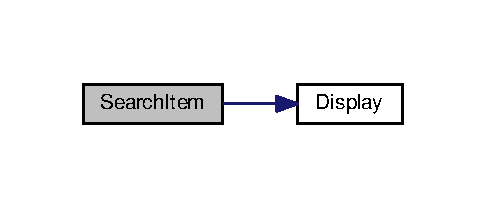
\includegraphics[width=233pt]{SelfOrganizing_8cpp_ad3123efb060bc3f8c45bd4f15b25bf3e_cgraph}
\end{center}
\end{figure}



%--- End generated contents ---

% Index
\backmatter
\newpage
\phantomsection
\clearemptydoublepage
\addcontentsline{toc}{chapter}{Index}
\printindex

\end{document}
